% MindBox Companion — Product Overview & Design Decisions
% Compile: pdflatex MindBox-Product-Overview.tex (run twice for TOC)
% Recommended: upload to Overleaf if local TeX packages are incomplete.

\documentclass[11pt,a4paper]{article}

\usepackage[utf8]{inputenc}
\usepackage[T1]{fontenc}
\usepackage{lmodern}
\usepackage[margin=2.5cm]{geometry}
\usepackage{hyperref}
\usepackage{xcolor}
\usepackage{booktabs}
\usepackage{longtable}
\usepackage{enumitem}
\usepackage{listings}
\usepackage{tikz}
\usetikzlibrary{arrows.meta, positioning, shapes.geometric, fit, backgrounds, calc}

\hypersetup{
  colorlinks=true,
  linkcolor=blue!70!black,
  urlcolor=blue!70!black,
  citecolor=blue!70!black,
  pdftitle={MindBox Companion — Product Overview},
}

\definecolor{codebg}{RGB}{245,245,245}
\definecolor{keyword}{RGB}{0,80,160}
\definecolor{decisionbg}{RGB}{240,248,255}

\lstset{
  basicstyle=\ttfamily\small,
  backgroundcolor=\color{codebg},
  frame=single,
  rulecolor=\color{gray!40},
  breaklines=true,
  columns=fullflexible,
  showstringspaces=false
}

\newcommand{\filepath}[1]{\texttt{#1}}
\newcommand{\designbox}[2]{%
  \noindent\fcolorbox{blue!40}{decisionbg}{%
    \parbox{\dimexpr\linewidth-2\fboxsep-2\fboxrule}{%
      \textbf{Design decision:} #1\\[0.3em]#2}}%
  \vspace{0.6em}}

\title{\textbf{MindBox Companion}\\[0.5em]
\large Product Overview \& Design Decisions\\[0.3em]
\normalsize Web Application (Study Assistor / IoT Focus Project)}
\author{MindBox Companion Team}
\date{\today}

\begin{document}
\maketitle

\begin{abstract}
This document is a single reference for the \textbf{MindBox Companion web application}:
what the product is for, who it serves, how it is built, and---most importantly---\emph{why}
key design choices were made. It covers the application layer only (React + TanStack Start +
Supabase); the ESP32 firmware is referenced where it affects app behaviour but is not
documented in depth here. Written for coursework reports, demos, and viva preparation.
\end{abstract}

\tableofcontents
\newpage

%==============================================================================
\section{Product Vision}
%==============================================================================

\subsection{Problem}

University students struggle to maintain consistent focus, understand \emph{when} they work
best, and balance coursework load with recovery. A desk device can capture honest focus
sessions and environmental context; a companion app can turn that data into history,
analytics, planning, and optional accountability---without replacing the physical ritual of
starting a session on the device.

\subsection{Solution}

\textbf{MindBox} is a physical focus timer with sensors (noise, light, temperature,
presence). \textbf{MindBox Companion} is the web app that:

\begin{itemize}[leftmargin=*]
  \item syncs and displays focus sessions from the device (or a dev simulator);
  \item provides analytics, wellbeing pattern estimates, and exports;
  \item lets students plan their semester (calendar, courses, exams);
  \item supports social motivation (friends, leaderboard) and read-only reviewer access
        (parents, mentors, supervisors);
  \item handles device pairing, telemetry, and optional email notifications.
\end{itemize}

\subsection{Product boundary}

\begin{table}[h]
\centering
\small
\begin{tabular}{@{}p{5.5cm}p{5.5cm}@{}}
\toprule
\textbf{Device (ESP32)} & \textbf{Companion app (this repo)} \\
\midrule
Start/stop focus timer & View history; no remote start/stop \\
Read sensors; drive LEDs & Charts, insights, calendar \\
Upload sessions via Wi-Fi & Auth, friends, reviewers, exports \\
Pair with user via code & Pairing UI + ingest API \\
\bottomrule
\end{tabular}
\caption{Clear separation of responsibilities}
\end{table}

\designbox{Device-first session control}{Sessions are \textbf{started and stopped on the
MindBox}, not from the web app. The companion is for reflection, planning, and sharing---not
for replacing the hardware interaction. This keeps the IoT story honest and avoids the app
becoming ``just another Pomodoro timer.''}

%==============================================================================
\section{Users and Roles}
%==============================================================================

\begin{description}[style=nextline, leftmargin=2.4cm]
  \item[Student (owner)] Primary user. Owns devices, sessions, settings, calendar, friends.
  \item[Friend] Another student with a MindBox account. Can send/accept friend requests;
        appears on weekly leaderboard (focus minutes among friends).
  \item[Reviewer] Invited by email with read-only grant. Can view a student's sessions,
        insights, and exports via a student picker---cannot edit their data.
  \item[Device / simulator] Not a human user, but an actor that POSTs to \filepath{/ingest/*}
        with a shared secret---no Supabase login.
\end{description}

All human roles share one authentication system (Supabase Auth: email/password or Google OAuth).

%==============================================================================
\section{Feature Overview}
%==============================================================================

The app exposes \textbf{15 routes}. Table~\ref{tab:features} maps each area to its purpose.

\begin{table}[h]
\centering
\small
\caption{Application feature map}
\label{tab:features}
\begin{tabular}{@{}llp{6.8cm}@{}}
\toprule
\textbf{Route} & \textbf{Area} & \textbf{Capability} \\
\midrule
\filepath{/} & Dashboard & Today's focus vs goal, streak, device state, insight teaser, recent sessions \\
\filepath{/calendar} & Planning & Month view, week strip, day timeline; courses (lecture/tutorial/lab), exams, semester bounds \\
\filepath{/history} & Sessions & Date range, charts, session list, reviewer student scope \\
\filepath{/session/:id} & Detail & Focus-load time series, environment samples, metadata \\
\filepath{/insights} & Analytics & Correlations, heatmaps, trends; wellbeing panel (recovery, circadian, routine) \\
\filepath{/leaderboard} & Social & Weekly minutes + streak among accepted friends \\
\filepath{/friends} & Social & Friend requests by email; optional notification email \\
\filepath{/reviewers} & Sharing & Invite/revoke read-only grants; accept via token link \\
\filepath{/exports} & Reports & CSV, JSON, printable HTML, email PDF to user + reviewers \\
\filepath{/device} & Hardware & 6-digit pairing, telemetry card, Web Bluetooth stub \\
\filepath{/simulator} & Development & In-browser fake device (seed sessions, telemetry) \\
\filepath{/settings} & Preferences & Profile, goals, nudges, quiet hours, external load, semester \\
\filepath{/login} & Auth & Sign in / sign up; Google OAuth \\
\filepath{/auth/callback} & Auth & OAuth redirect handler \\
\filepath{/reviewer/accept} & Auth & Accept reviewer invitation \\
\bottomrule
\end{tabular}
\end{table}

\textbf{Cross-cutting:} motivation nudges (inactivity + quiet hours), reduce-motion preference,
Focus Load Estimate on every session, weekly PDF auto-share when enabled.

%==============================================================================
\section{System Architecture}
%==============================================================================

\subsection{Pattern}

\begin{quote}
\textbf{Full-stack monolith + Backend-as-a-Service (BaaS) + thin custom server layer.}
\end{quote}

\begin{itemize}[leftmargin=*]
  \item \textbf{Monolith} --- one repository, one build, one deployable unit (simpler for a student team than microservices).
  \item \textbf{BaaS (Supabase)} --- PostgreSQL, authentication, Row-Level Security; no self-managed database server.
  \item \textbf{Thin server} --- custom HTTP entry (\filepath{server.ts}) for device ingest; TanStack \textbf{server functions} for email, pairing, privileged friend/reviewer logic.
\end{itemize}

\subsection{Architecture diagram}

\begin{center}
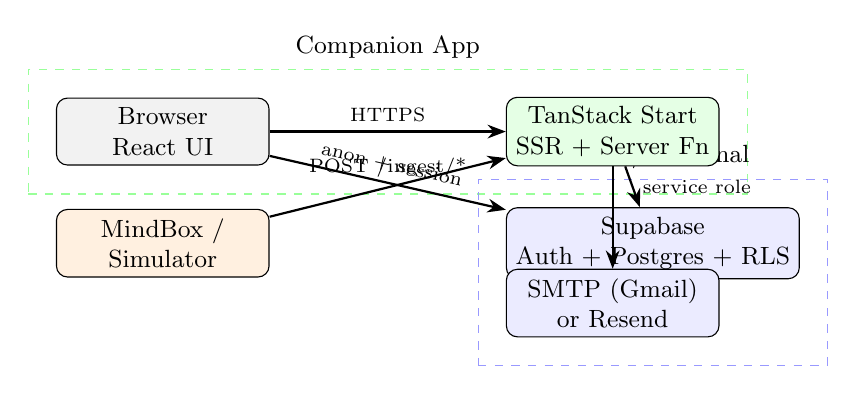
\begin{tikzpicture}[
  node distance=0.55cm and 1.1cm,
  box/.style={draw, rounded corners, minimum width=2.7cm, minimum height=0.85cm, align=center, font=\small},
  cloud/.style={box, fill=blue!8},
  app/.style={box, fill=green!10},
  device/.style={box, fill=orange!12},
  user/.style={box, fill=gray!10}
]
  \node[user] (browser) {Browser\\React UI};
  \node[device, below=of browser] (esp) {MindBox /\\Simulator};
  \node[app, right=3cm of browser] (app) {TanStack Start\\SSR + Server Fn};
  \node[cloud, right=3cm of esp] (supa) {Supabase\\Auth + Postgres + RLS};
  \node[cloud, below=1.3cm of app] (mail) {SMTP (Gmail)\\or Resend};

  \draw[-{Stealth}, thick] (browser) -- node[above, font=\scriptsize]{HTTPS} (app);
  \draw[-{Stealth}, thick] (browser) -- node[above, font=\scriptsize, sloped]{anon + session} (supa);
  \draw[-{Stealth}, thick] (esp) -- node[above, font=\scriptsize]{POST /ingest/*} (app);
  \draw[-{Stealth}, thick] (app) -- node[right, font=\scriptsize]{service role} (supa);
  \draw[-{Stealth}, thick] (app) -- (mail);

  \begin{scope}[on background layer]
    \node[fit=(browser)(app), draw=green!40, dashed, inner sep=10pt,
          label={[font=\small]above:Companion App}] {};
    \node[fit=(supa)(mail), draw=blue!40, dashed, inner sep=10pt,
          label={[font=\small]above:Cloud / External}] {};
  \end{scope}
\end{tikzpicture}
\end{center}

\subsection{Communication paths}

\begin{enumerate}[leftmargin=*]
  \item \textbf{Browser $\rightarrow$ Supabase} (direct): most reads/writes using the public anon key; RLS enforces ownership.
  \item \textbf{Browser $\rightarrow$ server functions}: privileged operations (device claim, friend email lookup, reviewer invites, PDF email).
  \item \textbf{Device $\rightarrow$ /ingest/*}: JSON upload with \texttt{x-device-secret}; no user JWT.
  \item \textbf{Server $\rightarrow$ SMTP/Resend}: transactional email (friends, reviewers, PDF reports).
\end{enumerate}

%==============================================================================
\section{Design Decisions}
%==============================================================================

This section records the main \textbf{why} behind the architecture. Use it in reports and
oral exams.

%------------------------------------------------------------------------------
\subsection{Platform and structure}
%------------------------------------------------------------------------------

\designbox{Supabase instead of a custom backend}{Managed Postgres + auth + RLS lets a small
team focus on product features (calendar, insights, ingest) instead of operating database
servers. Trade-off: vendor dependency and manual SQL migrations in the Supabase dashboard.}

\designbox{TanStack Start over separate frontend + API}{One TypeScript codebase, shared types,
SSR, and \texttt{createServerFn} RPCs reduce glue code. Trade-off: framework coupling and a
steeper learning curve than plain Create React App.}

\designbox{File-based routing (\filepath{src/routes/})}{Each URL maps to one file
(\filepath{history.tsx} $\rightarrow$ \filepath{/history}). Predictable for contributors;
TanStack Router generates \filepath{routeTree.gen.ts} automatically.}

\designbox{Logic in \filepath{lib/}, thin routes}{Pages compose UI; \filepath{lib/queries/},
\filepath{lib/insights.ts}, \filepath{lib/schedule.ts}, etc.\ hold testable domain logic.
Routes should not contain heavy algorithms.}

%------------------------------------------------------------------------------
\subsection{Security and data access}
%------------------------------------------------------------------------------

\designbox{Row-Level Security (RLS) as the primary guard}{Even if the browser anon key is
public, PostgreSQL policies restrict rows to \texttt{auth.uid()}. Defense in depth: server
functions still re-check \texttt{getUser()} before privileged actions.}

\designbox{Two Supabase clients}{Browser: anon key + user session. Server: cookie-bound user
client for RLS-aware ops; \textbf{service-role} client only in \filepath{*.server.ts} for
ingest and admin lookups. Service-role key never ships to the client.}

\designbox{Device ingest uses a shared secret, not user login}{The ESP32 cannot OAuth as the
student. Trust model: physical possession of device id + \texttt{DEVICE\_INGEST\_SECRET}.
Constant-time secret comparison prevents timing leaks.}

\designbox{Reviewer grants are read-only}{Reviewers get scoped SELECT via \texttt{reviewer\_grants}
and RPCs like \texttt{get\_reviewer\_students}---not co-ownership of the account. Streak RPC
(\filepath{0004\_streak\_access.sql}) explicitly authorizes reviewer access.}

\designbox{SECURITY DEFINER RPCs with narrow contracts}{Functions like \texttt{find\_profile\_by\_email}
and \texttt{get\_leaderboard} run as definer but filter by caller identity---needed where RLS
alone would block legitimate cross-user lookups (friend by email).}

%------------------------------------------------------------------------------
\subsection{Device integration}
%------------------------------------------------------------------------------

\designbox{Idempotent session upsert}{Devices may retry uploads. Upsert on
(\texttt{device\_id}, \texttt{session\_id}) ensures duplicates do not inflate history.
Child sample tables are replaced atomically per session.}

\designbox{Zod validation on ingest}{Incoming JSON is parsed with the same shape as
\filepath{focus-load.ts}. Firmware, simulator, and server share one contract.}

\designbox{Simulator as first-class dev path}{\filepath{scripts/simulator.ts} and
\filepath{/simulator} page mirror production ingest so the app is demoable without hardware.
Trade-off: simulator remains in production navigation (acceptable for coursework; hide for
public launch).}

\designbox{Web Bluetooth contract documented, not required}{\filepath{lib/bluetooth/web-bluetooth.ts}
defines GATT services for future direct pairing; primary path remains Wi-Fi ingest + 6-digit
code.}

%------------------------------------------------------------------------------
\subsection{Analytics and wellbeing}
%------------------------------------------------------------------------------

\designbox{Focus Load Estimate (FLE) is a heuristic, not a biometric}{Combines session
progress, noise, light stability, and presence interruptions into 0--100. Always labeled
``estimate'' in UI (\filepath{focus-load.ts}). Avoids false medical claims.}

\designbox{Three wellbeing signals, not a ``burnout score''}{Recovery balance, circadian
alignment, and routine consistency (\filepath{wellbeing.ts}) cite research but are explicitly
\textbf{behavioral pattern} indicators with confidence levels and transparent factors.
Non-clinical disclaimers in code and UI.}

\designbox{External load separate from calendar}{Settings ``Other commitments'' (hours/week
for lectures/labs) feeds \textbf{Recovery balance} in Insights---aggregate load, not timetable
slots. Calendar (\filepath{schedule\_events}) handles \textbf{when} classes happen; external
load handles \textbf{how much} non-MindBox demand exists.}

\designbox{Pure functions + Vitest}{Insights, schedule expansion, streak, dates, export
serialization, and wellbeing math live in testable modules (64+ unit tests). UI and server
integration are not yet covered by automated tests---documented limitation.}

%------------------------------------------------------------------------------
\subsection{Calendar and semester planning}
%------------------------------------------------------------------------------

\designbox{Weekly events expanded in application code, not SQL}{Recurring classes store
\texttt{day\_of\_week} + times; \filepath{expandScheduleEvents()} projects them onto calendar
days, optionally bounded by \texttt{semester\_start/end} on \filepath{user\_settings}
(migration \filepath{0008}). Keeps queries simple; logic is unit-tested.}

\designbox{Course builder $\rightarrow$ many \texttt{schedule\_events}}{One course (name, code,
color) expands to multiple rows: weekly lecture/tutorial/lab meetings + one-off exams
(\filepath{buildCourseEvents()} in \filepath{schedule.ts}). Easier editing than one row per
course with JSON blobs.}

\designbox{Exams as first-class category}{\texttt{category = exam} (migration \filepath{0008})
enables distinct styling, countdown widgets (\filepath{upcomingExams()}), and rose colour
--- separate from weekly classes.}

\designbox{Day timeline merges courses + focus sessions}{\filepath{buildDayAgenda()} interleaves
schedule occurrences with MindBox sessions so the calendar is the student's single daily
view---planning and actual focus side by side.}

%------------------------------------------------------------------------------
\subsection{Social, sharing, and email}
%------------------------------------------------------------------------------

\designbox{Friend requests require existing accounts}{Lookup by email via RPC; no invite-to-sign-up
flow. Reduces spam and keeps leaderboard data meaningful.}

\designbox{Friend notifications via server function}{Email lookup needs service-role; insert
uses user's RLS session. \filepath{friends.functions.ts} orchestrates both.}

\designbox{Gmail SMTP preferred over Resend for coursework}{Students often lack a custom domain.
\texttt{SMTP\_USER} + App Password (\filepath{send-html.server.ts}) sends to any address;
Resend sandbox only emails the account owner. SMTP tried first when configured.}

\designbox{PDF reports: HTML template $\rightarrow$ Puppeteer}{Email PDF matches on-site print
layout (\filepath{build-report-pdf.server.ts}). pdfkit fallback if headless Chrome unavailable.}

\designbox{Weekly share triggered from dashboard mount}{When enabled, \filepath{maybeSendWeeklySummaries()}
runs once per browser session. Simple for coursework; production would use a cron/edge job
(idempotent via \texttt{last\_weekly\_share\_at}).}

%------------------------------------------------------------------------------
\subsection{UX and accessibility}
%------------------------------------------------------------------------------

\designbox{URL search params for shareable filters}{History and insights encode date range and
reviewer student in the URL---bookmarkable views.}

\designbox{Reduce motion respected}{\filepath{ReduceMotionRoot} reads user setting; limits
animations for vestibular accessibility.}

\designbox{Motivation nudges with quiet hours}{Inactivity detection respects user quiet window
and master toggle---notifications are opt-in friendly.}

\designbox{Local calendar dates, not UTC midnight bugs}{\filepath{dates.ts} uses local
\texttt{YYYY-MM-DD} keys for filters and charts---fixes timezone off-by-one errors.}

%==============================================================================
\section{Technology Stack}
%==============================================================================

\begin{table}[h]
\centering
\small
\begin{tabular}{@{}lll@{}}
\toprule
\textbf{Layer} & \textbf{Choice} & \textbf{Rationale} \\
\midrule
Language & TypeScript & Shared types across UI, server, ingest \\
UI & React 19 & Component model, ecosystem \\
Routing & TanStack Router & Type-safe links, file-based routes \\
Data cache & TanStack Query & Server state, loading/error UX \\
Framework & TanStack Start & SSR + server functions in one project \\
Build & Vite 7 & Fast dev, modern bundling \\
Styling & Tailwind CSS 4 & Utility-first layout \\
Components & Radix / shadcn & Accessible primitives \\
Charts & Recharts & History, insights, session detail \\
Validation & Zod & Forms, ingest, server functions \\
Database & Supabase (PostgreSQL) & Auth, RLS, RPCs \\
Email & nodemailer (SMTP) + Resend fallback & Student-friendly sending \\
PDF & Puppeteer + pdfkit & Report attachments \\
Tests & Vitest & Pure logic unit tests \\
\bottomrule
\end{tabular}
\end{table}

%==============================================================================
\section{Database Schema}
%==============================================================================

Nine migrations (\filepath{0001}--\filepath{0009}) are applied manually in the Supabase SQL
Editor, then \texttt{NOTIFY pgrst, 'reload schema';}.

\subsection{Migration timeline}

\begin{table}[h]
\centering
\small
\begin{tabular}{@{}cl@{}}
\toprule
\textbf{File} & \textbf{Adds} \\
\midrule
\filepath{0001\_init.sql} & Core tables, RLS, \texttt{get\_leaderboard}, profile trigger \\
\filepath{0002\_app\_features.sql} & Friend RPCs, adaptive coaching column \\
\filepath{0003\_app\_gaps.sql} & Streak RPC, reviewer students, weekly share timestamp \\
\filepath{0004\_streak\_access.sql} & Secure streak for reviewer scope \\
\filepath{0005\_google\_oauth\_profile.sql} & Google display names on signup \\
\filepath{0006\_external\_load.sql} & External commitments $\rightarrow$ wellbeing \\
\filepath{0007\_schedule\_events.sql} & Calendar events table \\
\filepath{0008\_schedule\_exams\_semester.sql} & Exam category, semester dates on settings \\
\filepath{0009\_schedule\_subtype.sql} & Lecture / tutorial / lab subtype \\
\bottomrule
\end{tabular}
\end{table}

\subsection{Tables (13)}

\begin{itemize}[leftmargin=*]
  \item \texttt{profiles}, \texttt{user\_settings} --- user identity and preferences
  \item \texttt{devices}, \texttt{device\_profiles}, \texttt{device\_pairing\_codes}, \texttt{device\_status} --- hardware
  \item \texttt{sessions}, \texttt{focus\_load\_samples}, \texttt{env\_samples} --- focus data
  \item \texttt{friendships} --- social graph
  \item \texttt{reviewer\_grants} --- read-only sharing
  \item \texttt{external\_loads} --- aggregate non-MindBox load
  \item \texttt{schedule\_events} --- calendar (classes + exams)
\end{itemize}

\subsection{Key RPCs}

\texttt{get\_leaderboard}, \texttt{get\_focus\_streak}, \texttt{get\_reviewer\_students},
\texttt{get\_friends}, \texttt{find\_profile\_by\_email}.

%==============================================================================
\section{Critical Data Flows}
%==============================================================================

\subsection{Authentication (Google OAuth)}

Login $\rightarrow$ Supabase OAuth $\rightarrow$ Google $\rightarrow$ \filepath{/auth/callback}
$\rightarrow$ session cookies $\rightarrow$ \texttt{handle\_new\_user} trigger creates profile
$\rightarrow$ \texttt{AuthGate} allows app shell.

\subsection{Session sync (device)}

Firmware builds \texttt{SessionPayload} $\rightarrow$ POST \filepath{/ingest/sessions} +
secret $\rightarrow$ \filepath{ingest.server.ts} validates $\rightarrow$ admin upsert
$\rightarrow$ user sees data via React Query refetch.

\subsection{Calendar day view}

Load \texttt{schedule\_events} + sessions $\rightarrow$ \texttt{expandScheduleEvents()} for month/week
$\rightarrow$ \texttt{buildDayAgenda(selectedDate)} $\rightarrow$ timeline UI.

\subsection{Email PDF export}

User selects range on \filepath{/exports} $\rightarrow$ server function $\rightarrow$
load sessions $\rightarrow$ HTML report $\rightarrow$ Puppeteer PDF $\rightarrow$
\texttt{sendEmail()} to user + active reviewers.

%==============================================================================
\section{Project Structure (Application Code)}
%==============================================================================

\begin{lstlisting}
mindbox-companion-forge-main/
  src/
    server.ts              # HTTP entry: ingest routes, then SSR
    start.ts               # CSRF + error middleware
    routes/                # Pages (15 routes)
    components/            # App UI + shadcn primitives
    hooks/                 # useSessionScope, useMotivationNudge, ...
    lib/
      auth/                # AuthProvider, Google OAuth
      supabase/            # Browser + server + admin clients
      queries/             # React Query hooks
      api/                 # Server functions (*.functions.ts)
      ingest/              # Device upload handler
      email/               # SMTP, PDF, report delivery
      schedule.ts          # Calendar expansion + course builder
      wellbeing.ts         # Wellbeing estimators
      insights.ts          # Analytics helpers
      focus-load.ts        # FLE heuristic + ingest schema
      __tests__/           # Vitest (64 tests)
  supabase/migrations/     # SQL schema (0001-0009)
  scripts/                 # CLI simulator, cleanup
  docs/                    # This document + architecture guide
\end{lstlisting}

%==============================================================================
\section{Testing Strategy}
%==============================================================================

\begin{itemize}[leftmargin=*]
  \item \textbf{What is tested:} pure domain logic (wellbeing, insights, schedule, streak,
        dates, export, focus-load, quiet-hours, sensor-health, session-scope).
  \item \textbf{What is not tested (yet):} React components, server functions, ingest HTTP
        endpoints, RLS policies, email delivery.
  \item \textbf{Manual QA:} simulator seeds 30 days of data; pairing flow on \filepath{/device}.
  \item \textbf{Recommended next step:} one ingest integration test + GitHub Actions running
        \texttt{npm test} and \texttt{npm run build}.
\end{itemize}

%==============================================================================
\section{Configuration}
%==============================================================================

Copy \filepath{.env.example} to \filepath{.env}. Essential variables:

\begin{table}[h]
\centering
\small
\begin{tabular}{@{}ll@{}}
\toprule
\textbf{Variable} & \textbf{Purpose} \\
\midrule
\texttt{VITE\_SUPABASE\_URL}, \texttt{VITE\_SUPABASE\_ANON\_KEY} & Public Supabase (browser) \\
\texttt{SUPABASE\_SERVICE\_ROLE\_KEY} & Server-only admin (ingest, lookups) \\
\texttt{APP\_BASE\_URL} & Links in emails and OAuth redirects \\
\texttt{DEVICE\_INGEST\_SECRET} & Device/simulator ingest auth \\
\texttt{SMTP\_*} & Gmail (or other) outbound email \\
\texttt{RESEND\_*} & Optional email fallback \\
\bottomrule
\end{tabular}
\end{table}

Restart \texttt{npm run dev} after changing secrets.

%==============================================================================
\section{Known Limitations and Future Work}
%==============================================================================

\begin{table}[h]
\centering
\small
\begin{tabular}{@{}p{4.2cm}p{7.5cm}@{}}
\toprule
\textbf{Area} & \textbf{Current state / improvement} \\
\midrule
ESP32 firmware & Not in this repo; app tested via simulator \\
Supabase types & Placeholder \filepath{types.ts}; should run \texttt{supabase gen types} \\
CI/CD & No automated pipeline in repo \\
Integration tests & Ingest, RLS, email untested automatically \\
Weekly email job & Client-triggered; should be scheduled server-side \\
Simulator in nav & Dev tool visible to all users \\
Settings toggles & Haptics/adaptive coaching stored; device firmware applies them \\
Bluetooth pairing & Documented GATT; not production-complete \\
Battery UI & Feature-flagged off (\filepath{BATTERY\_TRACKING\_ENABLED}) \\
\bottomrule
\end{tabular}
\end{table}

%==============================================================================
\section{Evaluation Context (Coursework)}
%==============================================================================

For a computer science IoT + full-stack project, this application demonstrates:

\begin{itemize}[leftmargin=*]
  \item \textbf{Breadth} --- auth, social, analytics, calendar, IoT ingest, email, PDF.
  \item \textbf{Depth} --- RLS, idempotent ingest, researched wellbeing heuristics, tested schedule math.
  \item \textbf{Coherence} --- device-first product story; calendar + focus + insights form one student workflow.
\end{itemize}

In an era of AI-assisted coding, \textbf{feature count alone is not distinctive}; understanding
and being able to explain the design decisions in Section~4 \emph{is}. This document is
intended to support that explanation.

%==============================================================================
\section{Quick Reference Commands}
%==============================================================================

\begin{lstlisting}
npm install
npm run dev          # http://localhost:8080
npm run build
npm test             # 64 unit tests
npm run simulate     # CLI fake device (dev server must run)
npm run cleanup      # Remove simulator seed data
\end{lstlisting}

%==============================================================================
\section{Related Documents}
%==============================================================================

\begin{itemize}[leftmargin=*]
  \item \filepath{docs/MindBox-System-Architecture.tex} --- shorter student-friendly architecture guide with glossary.
  \item \filepath{README.md} --- setup steps and migration order.
  \item \filepath{supabase/migrations/} --- authoritative schema definitions.
\end{itemize}

%==============================================================================
\section{Summary}
%==============================================================================

MindBox Companion is a \textbf{TypeScript full-stack web application} built as a monolith on
\textbf{Supabase}, with a \textbf{custom ingest layer} for IoT devices. Its design prioritizes:
(1)~device-first focus capture, (2)~database-enforced security via RLS, (3)~testable domain
logic for analytics and planning, (4)~honest labeling of estimates, and (5)~student-realistic
operations (Gmail SMTP, simulator, manual migrations).

The three flows that unlock the rest of the system are \textbf{login}, \textbf{device ingest},
and \textbf{session fetch with RLS}. Calendar, social features, reviewers, and exports all
extend those foundations.

\vspace{1em}
\noindent\textbf{Document:} \filepath{docs/MindBox-Product-Overview.tex} \quad
\textbf{Application path:} \filepath{mindbox-companion-forge-main} \quad
\textbf{Version:} reflects migrations \filepath{0001}--\filepath{0009} and current feature set.

\end{document}
